The relative protection curves are in Figure \ref{fig:kiddyvaxmain-prot-rel-lr-boot}. The same considerations regarding the unjustified assumption of baseline risk of 1 apply here as they did with Ha Nam (Figure \ref{fig:kiddyvax-main-titre} shows many uninfected subjects with undetectable titres).

\begin{figure}[htp]
	\centering
	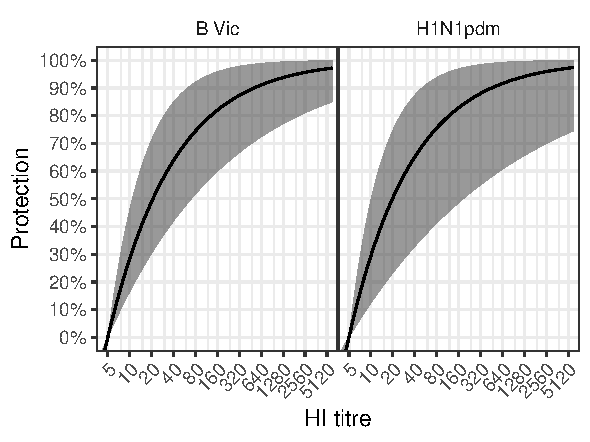
\includegraphics[width=0.8\textwidth]{../fit-logistic-boot-plot/kiddyvaxmain-prot-rel.pdf}
	\caption{
	Fitted relative-to-5 protection curves and confidence intervals from the standard logistic model fit to H1N1pdm and H3N2 subsets of kiddyvax data (shown in Figure \ref{fig:kiddyvax-main-titre}) using maximum likelihood with no accounting of censored titres (observations of 5 (below detectable) were unchanged, all other observations were moved to the midpoints of the corresponding censored intervals on a log scale). The solid line is the point estimates. The shaded region is the 95\% confidence interval. The bounds for the confidence interval were obtained by using the bootstrap method (10,000 samples).
	}
	\label{fig:kiddyvaxmain-prot-rel-lr-boot}
\end{figure}
